\documentclass{article}
\usepackage{indentfirst}
\usepackage{titling}
\usepackage{textpos}
\usepackage{tikz}
\usepackage{fancyhdr,graphicx,xcolor,colortbl}
\usepackage[explicit]{titlesec}
\usepackage{changepage}
\usepackage[toc,page]{appendix} 
\usepackage{float}
\usepackage{hyperref}
\usepackage[T1]{fontenc}
\usepackage{lstautogobble}
\usepackage{soul}
\usepackage{listings}
\usepackage{color}
\usepackage{textcomp}
\usepackage[T1]{fontenc}
\usepackage{caption}
\usepackage{hyperref}

\definecolor{jskeywords}{HTML}{8E44AD}% JavaScript keywords
\definecolor{jsextkeywords}{HTML}{006700}% JavaScript extended keywords

\definecolor{identifiers}{HTML}{645452} % identfiers 
\definecolor{string}{HTML}{B57281} % string literals
\definecolor{allcomment}{HTML}{808080} % comment

\definecolor{nodejs}{HTML}{629755} % Nodejs keywords 
\definecolor{testing}{HTML}{4169E1} % Node.js assert, jasmine
\definecolor{express}{HTML}{FF8C69} % Express.js
\definecolor{linenumber}{HTML}{996515} % line number
\definecolor{apricot}{HTML}{98777B} % numbers
\definecolor{linenofill}{HTML}{BEBEBE} % line number fill color
\definecolor{antiquefuchsia}{HTML}{915C83} % braces 
\definecolor{ballblue}{HTML}{21ABCD} % braces 

\definecolor{captioncolor}{rgb}{0.39, 0.33, 0.32} % caption color
\captionsetup[lstlisting]{font={color=captioncolor, small,tt}}

\captionsetup[lstlisting]{font={color=captioncolor, small, tt}}
\DeclareCaptionFormat{listing}{\rule{\dimexpr\textwidth+17pt\relax}{0.4pt}\vskip1pt#1#2#3}
\captionsetup[lstlisting]{format=listing,singlelinecheck=false, margin=0pt, font={sf},labelsep=space,labelfont=bf}

\lstdefinelanguage{JavaScript}{
  alsoletter={\\,.},
  keywords={arguments,await,break,case,catch,class,const,continue,debugger,default,delete,do,else,enum,eval,export,extends,false,finally,for,function,if,implements,import,in,instanceof,interface,let,new,null,package,private,protected,public,return,static,super,switch,this,throw,true,try,typeof,var,void,while,with,yield}, % JavaScript ES6 keywords
  keywordstyle=\color{jskeywords}\bfseries,
  ndkeywords={add, apply, args, Array, Array.from, Array.isArray, Array.of , Array.prototype, ArrayBuffer, bind, Boolean, call, charAt, charCodeAt, clear, codePointAt, concat, constructor, copyWithin, DataView, Date, Date.now, Date.parse, Date.prototype, Date.UTC, decodeURI, decodeURIComponent, encodeURI, encodeURIComponent, endsWith, entries, Error, Error.prototype, EvalError, every, false, fill, filter, find, findIndex, Float32Array, Float64Array, forEach, FulfillPromise, Function, Function.length, get, getDate, getDay, getFullYear, getHours, getMilliseconds, getMinutes, getMonth, getSeconds, getTime, getTimezoneOffset, getUTCDate, getUTCDay, getUTCFullYear, getUTCHours, getUTCMilliseconds, getUTCMinutes, getUTCMonth, getUTCSeconds, has,hasInstance, hasOwnProperty, ignoreCase, includes, indexOf, indexOf, Infinity, Int8Array, Int16Array, Int32Array, isConcatSpreadable, isFinite, isNaN, IsPromise, isPrototypeOf, Iterable, iterator, join, JSON, JSON.parse, JSON.stringify, keys, lastIndexOf, lastIndexOf, length, localeCompare, map, Map, Math, Math.abs , Math.acos, Math.acosh, Math.asin, Math.asinh, Math.atan, Math.atan2, Math.atanh, Math.cbrt, Math.ceil, Math.clz32, Math.cos, Math.cosh,  Math.E, Math.exp, Math.expm1, Math.floor, Math.fround, Math.hypot, Math.imul, Math.LN2, Math.LN10, Math.log, Math.log1p, Math.log2, Math.LOG2E, Math.log10, Math.LOG10E, Math.max, Math.min, Math.PI, Math.pow, Math.random, Math.round, Math.sign, Math.sin, Math.sinh, Math.sqrt, Math.SQRT1_2, Math.SQRT2, Math.tan, Math.tanh, Math.trunc, message, multiline, NaN, NewPromiseCapability, next, normalize, null, Number, Number.EPSILON, Number.isFinite, Number.isInteger, Number.isNaN, Number.isSafeInteger, Number.MAX_SAFE_INTEGER, Number.MAX_VALUE, Number.MIN_SAFE_INTEGER, Number.MIN_VALUE, Number.NaN, Number.NEGATIVE_INFINITY, Number.parseFloat, Number.parseInt, Number.POSITIVE_INFINITY, Number.prototype, Object, Object, Object.assign, Object.create, Object.defineProperties, Object.defineProperty, Object.freeze, Object.getOwnPropertyDescriptor, Object.getOwnPropertyNames, Object.getOwnPropertySymbols, Object.getPrototypeOf, Object.is, Object.isExtensible, Object.isFrozen, Object.isSealed, Object.keys, Object.preventExtensions, Object.prototype, Object.seal, Object.setPrototypeOf, of, parseFloat, parseInt, pop, Promise, Promise.all , Promise.race, Promise.reject, Promise.resolve, PromiseReactionJob, propertyIsEnumerable, prototype, Proxy, Proxy.revocable , push, RangeError, reduce, reduceRight, ReferenceError, Reflect, Reflect.apply, Reflect.construct , Reflect.defineProperty, Reflect.deleteProperty, Reflect.enumerate, Reflect.get, Reflect.getOwnPropertyDescriptor, Reflect.getPrototypeOf, Reflect.has, Reflect.isExtensible, Reflect.ownKeys, Reflect.preventExtensions, Reflect.set, Reflect.setPrototypeOf, Reflection, RegExp, RegExp, RegExp.prototype, repeat, replace, replace, reverse, search, search, Set, set, setDate, setFullYear, setHours, setMilliseconds, setMinutes, setMonth, setSeconds, setTime, setUTCDate, setUTCFullYear, setUTCHours, setUTCMilliseconds, setUTCMinutes, setUTCMonth, setUTCSeconds, shift, slice, slice, some, sort, species, splice, split, split, startsWith, String, String.fromCharCode, String.fromCodePoint, String.raw, substring, Symbol, Symbol.for, Symbol.hasInstance, Symbol.isConcatSpreadable, Symbol.iterator, Symbol.keyFor, Symbol.match, Symbol.prototype, Symbol.replace, Symbol.replace, Symbol.search, Symbol.species, Symbol.split, Symbol.toPrimitive, Symbol.toStringTag, Symbol.unscopables, SyntaxError, then, toDateString, toExponential, toFixed, toISOString, toJSON, toLocaleDateString, toLocaleLowerCase, toLocaleString, toLocaleString, toLocaleString, toLocaleString, toLocaleTimeString, toLocaleUpperCase, toLowerCase, toPrecision, toPrimitive, toString, toStringTag, toTimeString, toUpperCase, toUTCString, TriggerPromiseReactions, trim, true, TypeError, Uint8Array, Uint8ClampedArray, Uint16Array, Uint32Array, undefined, unscopables, unshift, URIError, valueOf, WeakMap, WeakSet
  }, % JavaScript extended keywords
  ndkeywordstyle=\color{jsextkeywords}\bfseries,
  identifierstyle=\color{identifiers},
  sensitive=true,
  stringstyle=\color{string}\ttfamily,
  morestring=[b]", 
  morestring=[d]',
  morestring=[s][\color{string}\ttfamily]{`}{`},
  commentstyle=\color{red}\itshape,
  morecomment=[l][\color{allcomment}]{//},
  morecomment=[s][\color{allcomment}]{/*}{*/},
  morecomment=[s][\color{allcomment}]{/**}{*/},
  emph={app.all, app.delete, app.disable, app.disabled, app.enable, app.enabled, app.engine, app.get, app.listen, app.locals, app.METHOD, app.mountpath, app.param, app.path, app.post, app.put, app.render, app.route, app.set, app.use, express, express.Router, express.static, req.acceptLanguages, req.accepts, req.acceptsCharsets, req.acceptsEncodings, req.app, req.baseUrl, req.body, req.cookies, req.fresh, req.get, req.hostname, req.ip, req.ips, req.is, req.method, req.originalUrl, req.param, req.params, req.path, req.protocol, req.query, req.range, req.route, req.secure, req.signedCookies, req.stale, req.subdomains, req.xhr, res.app, res.append, res.attachment, res.clearCookie, res.cookies, res.download, res.end, res.format, res.get, res.headersSent, res.json, res.jsonp, res.links, res.locals, res.location, res.redirect, res.render, res.sendFile, res.sendStatus, res.set, res.status, res.type, res.vary, router.all, router.METHOD, router.param, router.route, router.use}, % express keywords
  emph={[2]agent.createConnection, agent.destroy, agent.freeSockets, agent.getName, agent.maxFreeSockets, agent.maxSockets, agent.requests, agent.sockets, certificate.exportChallenge, certificate.exportPublicKey, certificate.verifySpkac, child.channel, child.connected, child.disconnect, child.kill, child.pid, child.send, child.stderr, child.stdin, child.stdio, child.stdout, child_process.exec, child_process.execFile, child_process.execFileSync, child_process.execSync, child_process.fork, child_process.spawn, child_process.spawnSync, cipher.final, cipher.getAuthTag, cipher.setAAD, cipher.setAutoPadding, cipher.update, clearImmediate, clearImmediate, clearInterval, clearInterval, clearTimeout, clearTimeout, console, console.assert, console.dir, console.error, console.info, console.log, console.time, console.timeEnd, console.trace, console.warn, decipher.final, decipher.setAAD, decipher.setAuthTag, decipher.setAutoPadding, decipher.update, dgram.createSocket, dgram.createSocket, diffieHellman.computeSecret, diffieHellman.generateKeys, diffieHellman.getGenerator, diffieHellman.getPrime, diffieHellman.getPrivateKey, diffieHellman.getPublicKey, diffieHellman.setPrivateKey, diffieHellman.setPublicKey, diffieHellman.verifyError, dns.getServers, dns.getServers, dns.lookup, dns.lookup, dns.lookupService, dns.resolve, dns.resolve4, dns.resolve6, dns.resolveCname, dns.resolveMx, dns.resolveNaptr, dns.resolveNs, dns.resolvePtr, dns.resolveSoa, dns.resolveSrv, dns.resolveTxt, dns.reverse, dns.setServers, ecdh.computeSecret, ecdh.generateKeys, ecdh.getPrivateKey, ecdh.getPublicKey, ecdh.setPrivateKey, ecdh.setPublicKey, error.address, error.code, error.errno, error.message, error.path, error.port, error.stack, error.syscall, exports, fs.access, fs.accessSync, fs.appendFile, fs.appendFileSync, fs.chmod, fs.chmodSync, fs.chown, fs.chownSync, fs.close, fs.closeSync, fs.constants, fs.createReadStream, fs.createWriteStream, fs.exists, global, http.createServer, http.get, http.globalAgent, http.request, https.createServer, https.get, https.globalAgent, https.request, message.destroy, message.headers, message.httpVersion, message.method, message.rawHeaders, message.rawTrailers, message.setTimeout, message.socket, message.statusCode, message.statusMessage, message.trailers, message.url, module, module.children, module.exports, module.filename, module.id, module.loaded, module.parent, module.require, os.arch, os.constants, os.cpus, os.endianness, os.EOL, os.freemem, os.homedir, os.hostname, os.loadavg, os.networkInterfaces, os.platform, os.release, os.tmpdir, os.totalmem, os.type, os.uptime, os.userInfo, path.basename, path.delimiter, path.dirname, path.extname, path.format, path.isAbsolute, path.join, path.normalize, path.parse, path.posix, path.relative, path.resolve, path.sep, path.win32, process, process.abort, process.arch, process.argv, process.argv0, process.channel, process.chdir, process.config, process.connected, process.cpuUsage, process.cwd, process.disconnect, process.emitWarning, process.env, process.execArgv, process.execPath, process.exit, process.exitCode, process.getegid, process.geteuid, process.getgid, process.getgroups, process.getuid, process.hrtime, process.initgroups, process.kill, process.mainModule, process.memoryUsage, process.nextTick, process.pid, process.platform, process.release, process.send, process.setegid, process.seteuid, process.setgid, process.setgroups, process.setuid, process.stderr, process.stdin, process.stdout, process.title, process.umask, process.uptime, process.version, process.versions, querystring.escape, querystring.parse, querystring.stringify, querystring.unescape, r.clearLine, readable.pause, readable.pipe, readable.push, readable.push, readable.read, readable.read, readable.resume, readable.setEncoding, readable.unpipe, readable.unshift, readable.wrap, readable._read, readStream.bytesRead, readStream.isRaw, readStream.path, readStream.setRawMode, repl.start, request.abort, request.aborted, request.end, request.flushHeaders, request.setNoDelay, request.setSocketKeepAlive, request.setTimeout, request.write, require, require.cache, require.extensions, response.addTrailers, response.end, response.finished, response.getHeader, response.getHeaderNames, response.getHeaders, response.hasHeader, response.headersSent, response.removeHeader, response.sendDate, response.setHeader, response.setTimeout, response.statusCode, response.statusMessage, response.write, response.writeContinue, response.writeHead, rl.clearScreenDown, rl.close, rl.createInterface, rl.cursorTo, rl.emitKeypressEvents, rl.moveCursor, rl.pause, rl.prompt, rl.question, rl.resume, rl.setPrompt, rl.write, script.runInNewContext, script.runInThisContext, server.addContext, server.address, server.address, server.close, server.close, server.connections, server.getTicketKeys, server.listen, server.listen, server.setTicketKeys, server.setTimeout, server.setTimeout, server.timeout, server.timeout, setImmediate, setInterval, setTimeout, socket.addMembership, socket.address, socket.bind, socket.bind, socket.close, socket.dropMembership, socket.ref, socket.send, socket.setBroadcast, socket.setMulticastLoopback, socket.setMulticastTTL, socket.setTTL, socket.unref, stream.Readable, stringDecoder.end, stringDecoder.write, timeout.ref, timeout.unref, tls.connect, tls.createSecureContext, tls.createServer, tls.getCiphers, tlsSocket.address, tlsSocket.authorizationError, tlsSocket.authorized, tlsSocket.encrypted, tlsSocket.getCipher, tlsSocket.getEphemeralKeyInfo, tlsSocket.getPeerCertificate, tlsSocket.getProtocol, tlsSocket.getSession, tlsSocket.getTLSTicket, tlsSocket.localAddress, tlsSocket.localPort, tlsSocket.remoteAddress, tlsSocket.remoteFamily, tlsSocket.remotePort, tlsSocket.renegotiate, tlsSocket.setMaxSendFragment, transform._flush, transform._transform, util.debuglog, util.deprecate, util.format, util.inherits, util.inspect, v8.getHeapStatistics, v8.setFlagsFromString, vm.createContext, vm.isContext, vm.runInContext, vm.runInDebugContext, vm.runInNewContext, vm.runInThisContext, watcher.close, worker.disconnect, worker.exitedAfterDisconnect, worker.id, worker.isConnected, worker.isDead, worker.kill, worker.process, worker.send, worker.suicide, writable.cork, writable.end, writable.setDefaultEncoding, writable.write, writeStream.bytesWritten, writeStream.columns, writeStream.path, writeStream.rows, zlib, zlib.createGunzip, zlib.createGzip, zlib.createInflate, zlib.createInflateRaw, zlib.createUnzip, zlib.deflate, zlib.deflateRaw, zlib.deflateRawSync, zlib.deflateSync, zlib.gunzip, zlib.gunzipSync, zlib.gzip, zlib.gzipSync, zlib.inflate, zlib.inflateRaw, zlib.inflateRawSync, zlib.inflateSync, zlib.unzip, zlib.unzipSync, __dirname, __filename}, % Node.js keywords
  emph={[3] assert, assert.deepEqual, assert.deepStrictEqual, assert.doesNotThrow, assert.equal, assert.fail, assert.ifError, assert.notDeepEqual, assert.notDeepStrictEqual, assert.notEqual, assert.notStrictEqual, assert.ok, assert.strictEqual, assert.throws, describe, toBe, it, xdescribe, beforeEach, afterEach, beforeAll, afterAll, expect, it, xit, xdiscribe, pending, and.callThrough, and.returnValue, and.returnValues, and.callFake, and.throwError, and.stub, .not, .calls.any, .calls.count, .calls.argsFor, .calls.allArgs, .calls.all, .calls.mostRecent, .calls.first, .calls.reset, jasmine.createSpy, jasmine.createSpyObj, jasmine.any, jasmine.anything, jasmine.objectContaining, jasmine.arrayContaining, jasmine.stringMatching, asymmetricMatch,  jasmine.clock, .not.toBeTruthy, .toBeTruthy, .not.toBeFalsy, .toBeFalsy, .not.toBeDefined .toBeDefined, .not.toBeNull .toBeNull, .not.toEqual .toEqual, .not.toBeCloseTo .toBeCloseTo, .not.toContain, .toContain, .not.toMatch, .toMatch, .not.toBeGreaterThan, .toBeGreaterThan, .not.toBeLessThan, .toBeLessThan, .toThrow, .not.toThrow, .toBeNull, .not.toBeNull, .toBeDefined, .not.toBeDefined}, % Node.js Assert, Jasmine, ... keywords
  }

  \lstset{
   basicstyle=\normalsize\linespread{1.1}\footnotesize\ttfamily,
   language=JavaScript,
   % frame=top,frame=bottom,
   breaklines=true,
   showstringspaces=false,
   tabsize=2,
   upquote = true,
   numbers=left, 
   numberstyle=\tiny, 
   stepnumber=1, 
   numbersep=5pt,
   numberblanklines=false,
   xleftmargin=17pt,
   framexleftmargin=17pt,
   framexrightmargin=17pt,
   framexbottommargin=5pt,
   framextopmargin=5pt,
   alsoother={.},
   captionpos=t,
   literate=
            *{\{}{{\textcolor{antiquefuchsia}{\{}}}{1}% punctuators 
            {\}}{{\textcolor{antiquefuchsia}{\}}}}{1}%
            {(}{{\textcolor{antiquefuchsia}{(}}}1%
            {)}{{\textcolor{antiquefuchsia}{)}}}1%
            {[}{{\textcolor{antiquefuchsia}{[}}}1%
            {]}{{\textcolor{antiquefuchsia}{]}}}1%
            {...}{{\textcolor{ballblue}{...}}}1%
            {;}{{\textcolor{antiquefuchsia}{;}}}1%
            {,}{{\textcolor{antiquefuchsia}{,}}}1%
            {>}{{\textcolor{ballblue}{>}}}1%
            {<}{{\textcolor{ballblue}{<}}}1%
            {<=}{{\textcolor{ballblue}{<=}}}1%
            {>=}{{\textcolor{ballblue}{>=}}}1%
            {==}{{\textcolor{ballblue}{==}}}1%
            {!=}{{\textcolor{ballblue}{!=}}}1%
            {===}{{\textcolor{ballblue}{===}}}1%
            {!==}{{\textcolor{ballblue}{!==}}}1%
            {+}{{\textcolor{ballblue}{+}}}1%
            {-}{{\textcolor{ballblue}{-}}}1%
            {*}{{\textcolor{ballblue}{*}}}1%
            {\%}{{\textcolor{ballblue}{\%}}}1%
            {++}{{\textcolor{ballblue}{++}}}1%
            {--}{{\textcolor{ballblue}{--}}}1%
            {<<}{{\textcolor{ballblue}{<<}}}1%
            {>>}{{\textcolor{ballblue}{>>}}}1%
            {>>>}{{\textcolor{ballblue}{>>>}}}1%
            {=}{{\textcolor{ballblue}{=}}}1%
            % {&}{{\textcolor{ballblue}{&}}}1%
            {|}{{\textcolor{ballblue}{|}}}1%
            {^}{{\textcolor{ballblue}{^}}}1%
            {!}{{\textcolor{ballblue}{!}}}1%
            {~}{{\textcolor{ballblue}{~}}}1%
            % {&&}{{\textcolor{ballblue}{&&}}}1%
            {||}{{\textcolor{ballblue}{||}}}1%
            {?}{{\textcolor{ballblue}{?}}}1%
            {:}{{\textcolor{ballblue}{:}}}1%
            {=}{{\textcolor{ballblue}{=}}}1%
            {+=}{{\textcolor{ballblue}{+=}}}1%
            {-=}{{\textcolor{ballblue}{-=}}}1%
            {*=}{{\textcolor{ballblue}{*=}}}1%
            {\%=}{{\textcolor{ballblue}{\%=}}}1%
            {<<=}{{\textcolor{ballblue}{<<=}}}1%
            {>>=}{{\textcolor{ballblue}{>>=}}}1%
            {>>>=}{{\textcolor{ballblue}{>>>=}}}1%
            {&=}{{\textcolor{ballblue}{&=}}}1%
            {|=}{{\textcolor{ballblue}{|=}}}1%
            {^=}{{\textcolor{ballblue}{^=}}}1%
            {=>}{{\textcolor{ballblue}{=>}}}1%
            {\\b}{{\textcolor{ballblue}{\textbackslash{}b}}}1% escape sequences
            {\\t}{{\textcolor{apricot}{\textbackslash{}t}}}{1}%
            {\\n}{{\textcolor{apricot}{\textbackslash{}n}}}{1}%
            {\\v}{{\textcolor{apricot}{\textbackslash{}v}}}{1}%
            {\\f}{{\textcolor{apricot}{\textbackslash{}f}}}{1}%
            {\\r}{{\textcolor{apricot}{\textbackslash{}r}}}{1}%
            {\\"}{{\textcolor{apricot}{\textbackslash{}"}}}{1}%
            {\\'}{{\textcolor{apricot}{\textbackslash{}'}}}{1}%
            {\\}{{\textcolor{apricot}{\textbackslash{}}}}{1}%
            {0}{{\textcolor{apricot}{0}}}{1}% numbers
            {1}{{\textcolor{apricot}{1}}}{1}%
            {2}{{\textcolor{apricot}{2}}}{1}%
            {3}{{\textcolor{apricot}{3}}}{1}%
            {4}{{\textcolor{apricot}{4}}}{1}%
            {5}{{\textcolor{apricot}{5}}}{1}%
            {6}{{\textcolor{apricot}{6}}}{1}%
            {7}{{\textcolor{apricot}{7}}}{1}%
            {8}{{\textcolor{apricot}{8}}}{1}%
            {9}{{\textcolor{apricot}{9}}}{1}%
            {.0}{{\textcolor{apricot}{.0}}}{2}%
            {.1}{{\textcolor{apricot}{.1}}}{2}% 
            {.2}{{\textcolor{apricot}{.2}}}{2}%
            {.3}{{\textcolor{apricot}{.3}}}{2}%
            {.4}{{\textcolor{apricot}{.4}}}{2}%
            {.5}{{\textcolor{apricot}{.5}}}{2}%
            {.6}{{\textcolor{apricot}{.6}}}{2}%
            {.7}{{\textcolor{apricot}{.7}}}{2}%
            {.8}{{\textcolor{apricot}{.8}}}{2}%
            {.9}{{\textcolor{apricot}{.9}}}{2},%
   emphstyle={\color{express}}, % express
   emphstyle={[2]\color{nodejs}}, % node.js
   emphstyle={[3]\color{testing}}, % jasmine ...
   numberstyle=\normalfont\tiny\textcolor{linenumber} % line number
}


\lstset{language=JavaScript}
\lstset{autogobble=true}


\title{Compiler Construction}

\date{\today}
\author{Lucas Franceschino}

\newcommand\cc[1]{\lstinline{#1}}
\newcommand\ccd[1]{\small\textcolor[HTML]{7D6557}{\texttt{#1}}}
\newcommand\todo{\begin{center}\textbf{»»»»»» ~~~~~ICI - TODO~~~~~ ««««««}\end{center}}

	
\begin{document}
	\maketitle
	\tableofcontents
	\newpage
	\section{Language choice}
		I chose to implement my compiler in \textbf{TypeScript}, which is a super-set of JavaScript. It offers ES6 support\footnote{ES6 is the new version of JS, support \cc{let}, \cc{arrow functions}, \cc{destructuring}, \cc{full class support}\dots. For more details, see \url{http://es6-features.org} }, static typing, generic typing, interfaces, union types\dots : it makes JavaScript much stricter and safer.

		The choice of that language is motivated mainly by the fact I actually use a lot JS for projects these days. It is a very flexible and nice to use language\footnote{\url{http://bdcampbell.net/javascript/book/javascript_the_good_parts.pdf} and \url{http://javascript.crockford.com/javascript.html}}. It has some "bad parts", but ES6 plus TypeScript makes them disappear.
	\section{Global design}
		This compiler is intended to be generic and not linked to SPL. Everything is split in two parts: the generic part and the SPL implementation. These statements are more or less true: for example, code generation jumps from the abstract syntax tree to SSM. Then, here no abstraction part is built, a direct SSM builder is used.
	\section{Lexer}
		The lexer is very simple: it processes the whole file and builds up a list of tokens. It does not support streams.
		
		In order to have a generic lexer, I have a few classes that the user needs to extend to implement an actual language:
		\begin{itemize}
			\item \textbf{Lexer:} is the base of a lexer. Basically, you extend that class, let's say, \cc{SPL\_Lexer}, and then you link tokens to it.
			\item \textbf{Token:} take care of everything related to tokens. When implementing a language, you extend Token as much as you have different tokens to be recognize.
			\item \textbf{DeterministicToken:}\label{detToken} a specific kind of \cc{Token}.
		\end{itemize}

		\subsection{How it works}
		The lexer takes an input string, then ask every registered tokens to try to match against the string, one by one by order of registration. If a token matches a string, then it is saved and the operation is repeated. Otherwise, we try another token. If no token matches, then, we raise an error.

		\subsection{Error management}
		When an error is raised, it is first constructed by a method in the \cc{Lexer} class: it takes in parameter some position in the original file, some length and a message, and format nicely a colored error.

		\subsection{Token and deterministic token}\label{explainToken}
		When adding a kind of Token, you provide just a regular expression, and optionally a paired token (for instance \cc{(} is paired to \cc{)} and \textit{vice versa}). Example of token declaration (supposing \cc{SPL_Lexer} is a defined lexer):

		\begin{lstlisting}
			export class Integer extends Token {}
			SPL_Lexer.register (Integer, /\b\d+\b/y);
		\end{lstlisting}

		Token provides the following methods:
		\begin{itemize}
			\item \cc{match}: as seen previously it tries to match against a string.
			\item \cc{generateRand}: generate a random string matching the regular expression of the token. This will be very useful to generate random programs.
			\item \cc{error}: it takes in parameter a message and display an error using the previously described \cc{Lexer} function.
		\end{itemize}

		\cc{DeterministicToken} is a normal token, but instead of having a regular expression, it has just a string, that's why it's qualified of deterministic. That is useful for pretty printing.

		An \cc{EOF} (\textit{end of file}) token is predefined and appends to the list of produced tokens by the Lexer. Then, when implementing a language, there is an standard way of representing \textit{end of file}.


		\subsection{Paired token}\label{pairedToken}
			Since a token can be declared as being a pair, the lexer also checks and links automatically paired tokens. Then, it avoids doing it later on when the parser will need it.

	\section{Parser}
		Again, the parser is general, and works for any given grammar.
		\subsection*{Note}
			What I presented in my slides during the first two presentations is "outdated": I rebuilt from the bottom my compiler. Indeed, before, the grammar was defined by a file using an intuitive representation looking like:
			 \begin{lstlisting}
			 	SPL			Decl+, 'eof'
			 	Decl		VarDecl | FunDecl as content
			 	VarDecl 	'var' | Type as type, 'id' as name, i '=', Exp as exp, i ';'
			 	FunDeclT	i '::', FunType
			 	RetType		Type | 'Void' #drop
			 	 ...
			 \end{lstlisting}
			But I chose to drop it, because it built some non-typed data. Now every rule as its own class, and everything is typed checked, hence everything is much more stable and exploitable. 
		\subsection{Architecture}
			Basically, everything is run by 3 classes:
			\begin{itemize}
				\item \cc{Parser}: global parser class.
				\item \cc{ParserRule}: represents a grammar rule. Each grammar rule is represented by extending that class. 
				\item \cc{ParserRuleStep}: represents a step of a grammar rule.
			\end{itemize}
		\subsection{Declaring a rule}
			Here is the declaration of \cc{VarType}, with \cc{SPL_Parser} a class extending \cc{Parser}:
			\label{VarTypeDef}\begin{lstlisting}
				export class VarDecl extends ParserRule{
					@SPL_Parser.addStep() 		type: LexSPL.Var | Type;
					@SPL_Parser.addStep() 		name: LexSPL.Id;
					@SPL_Parser.addIgnoreTokenStep( LexSPL.Equal )
							       .addStep() 		exp: Exp;
					@SPL_Parser.addIgnoreTokenStep( LexSPL.Semicolon )
				}
			\end{lstlisting}

			The decorators \cc{@SPL_Parser.add*} are there to declare that an attribute is intended to receive some tokens or some constructs. This way, it is easy to define a grammar rule, and to use it later on. Moreover, TypeScript is able to type check everything, and also to auto complete while dealing with such entities.

			One can define optional steps or repeated steps in the following way:
			
			\begin{lstlisting}
				@SPL_Parser.addStep() statements: Stmt[]; // one or more Stmt
				@SPL_Parser.addStep() statements?: Stmt[]; // any number of Stmt
				@SPL_Parser.addStep() annotation?: Annot; // zero or one annotation
			\end{lstlisting}

			It relies on TypeScript type annotation, but the sad thing is that Type reflection at run-time is not completely supported by TypeScript\footnote{\href{http://blog.wolksoftware.com/decorators-metadata-reflection-in-typescript-from-novice-to-expert-part-4}{blog.wolksoftware.com/decorators...}}. Basically, TypeScript can generate (on compilation time) some decorators to give run time information about types, but only for basic build-in ones: that library is not mature at all, so I made a little tweak to get it works. I use Grunt (a JavaScript task runner) to pre compile all my files, spot where \cc{addStep} is used and adds type information explicitly.

			From a \cc{Parser}, it is possible to add steps using either \cc{addStep} or \cc{addIgnoreTokenStep} decorator\footnote{https://www.typescriptlang.org/docs/handbook/decorators.html}. A step can be a Token or an instance of some ParserRule. An IgnoreTokenStep takes in parameter a \cc{DeterministicToken} (as defined in section \ref{detToken}).

			You can notice that \cc{addIgnoreTokenStep} is not bind to a class attribute. It makes sense: we don't want to have to name a field for recognizing \cc{;} for instance: \cc{;} is just a separator. Such a token does not contain any information, whereas an integer token would actually contain actual important information.

			Here comes the notion \cc{DeterministicToken}: it is deterministic, so that it is useless to store any information about any instance of such a token. But, while pretty-printing, we need to write something: there is a reason to have a semi-colon in a grammar, for instance.

		\subsection{Pretty printer}
			To pretty print an instance of a certain \cc{ParserRule}, it just needs to print the \cc{DeterministicToken}, to print the content of other tokens, and to recursively apply the same process to contained instances of \cc{ParserRule} (if any).

			There is the default way of generating the string representation of some \cc{ParserRule}, but it can be overridden. Moreover, the indentation is managed using two decorators: \cc{@ppIdent} and \cc{@ppNewLine}. \cc{@ppIdent} says that the string should be indented by one lever more, while \cc{@ppNewLine} says the string has to treated as a "block" more than as an inline thing.
		\subsection{Random program generator}
			A \cc{ParserRule} contains every information necessary to generate a random string corresponding to it. To do so, we just browse all declared steps, and generate random strings for each of them, and create an instance of that rule with the newly generated sub-rules or sub-tokens. If a step is optional, then we decide randomly to generate something or not, same thing if a step can be repeated.

			When all of that is done, just pretty print the resulting \cc{ParserRule}.


		\subsection{Parsing}
			As previously described, implementing a parser means:
			\begin{enumerate}
				\item have a class extending \cc{Parser}, say \cc{SPL_Parser};
				\item have one class per rule extending \cc{ParserRule}.  
			\end{enumerate}
			The parsing is initiated by \cc{SPL_Parser} from a token list. It gets the first declared rule, and makes it parse the token list. The token list is actually a \cc{TokenDeck}.
			\subsubsection{TokenDeck}
				A \cc{TokenDeck} contains a list of tokens. It has a list-like behaviour, but always keeps the whole list. It just keeps track of the position of the current token. The idea is to pass this \cc{TokenDeck} from \cc{TokenRule} to \cc{TokenRule}, and in the same time, keep the track of the attempts.
				If the main rule can't match anything, then it is very easy to find the most advanced attempts and display it.

			\subsubsection{\cc{Parser} internal parsing}
				Parsing a \cc{TokenDeck} $deck$ from a \cc{ParserRule} $pr$ means that we want $deck$ to "fit in" $pr$. $deck$ being recognized by $pr$ means that each steps of $pr$ can parse sequentially $deck$. 

				A step is a list of possible things to recognize. If any of them can recognize $deck$, then $deck$ is recognized by the step.

		\subsection{Grammar analysis \& optimization}
			Using the previously described method to parse a \cc{TokenDeck} is not very efficient: indeed, since it's all about recursive finding and backtracking, there are some situations where parsing is very inefficient.

			In order to speed up the process, we optimize the grammar rules.

			\subsubsection{Left recursion}
			Since left recursion leads to probable infinite loops, we need to detect it and avoid it.

			Before actually optimizing the grammar, we check for left recursion. If such a rule is found, the parser throws an exception.

			\subsubsection{Determine the n-th token to be accepted by a rule}
			I tried to make a function determining what tokens can be accepted by a parser at the n-th position, just by looking at the rule definitions, and I actually spent quite a lot of time on it.

			The idea was to use a tree, with all the possible acceptable tokens on the n-th level of that tree. I used a sort of shadow tree: it was actually updating sub-trees only when necessary, and keeping everything as references, to handle recursion (since the rules are themselves recursive).

			But after a few days of full work on that idea, I just got some almost working algorithms, but I always ended up having issues, like some tokens were missing from some places in the tree.

			I eventually decided to stop this experiment there, since it took me too much time already.  

			\subsubsection{First token}
			Instead of being able to predict the n-th possible tokens, I chose just to look up for the first possible tokens, which is very straightforward.

			Then, instead of trying each different possibility in a rule, it is now possible to test only the one with a matching first tokens.

			To optimize that, I use hash-tables from token kinds to possible rules for each step of each rule. Then, given a token, we get a list of possible rules to apply, and then we avoid testing anything but necessary things.

			\subsubsection{Paired tokens or how to have easy multiple errors handling}
			As explained in section \ref{explainToken}, a Token can be linked to another one to declare a pair. Since then, the parser treats these tokens as pair, hence, an opening something has to match with a closing something. The parser actually uses that fact.

			Indeed, when trying to parse in the context of some \cc{ParserRule} $pr$, if the parser detects a pair token, it matches its closing token, extracts\footnote{The extraction is immediate and in linear time, as explained in section \ref{pairedToken}, the matching is done previously by the lexer} the section and parses it independently.

			This only happens if - in the context of $pr$ - there is only one possible grammar rule that can recognize the pair expression.

			For instance, parsing \texttt{(3) + 4} when the only rule that can be applied is \texttt{Parenthesis = '(' Exp ')'}, \texttt{(3)} is extracted and parsed independently. Here, we know it has to match. If it doesn't match, we know that what was inside the parenthesis is wrong. Then, we raise an error, without stopping parsing. 

			\subsubsection{Paired token optimization}
			Consider the following expression \texttt{((\dots(3)\dots))}: we don't want the parser to do the usual backtracking thing here. Indeed, the rule \texttt{Parenthesis = '(' Exp ')'} consists of exactly 3 steps : opening, inside rule, closing. If the inside rule is not of this "opening inside closing" form, then we can just parse the expression in a linear way, but extracting \texttt{3}.

			\subsubsection{Same thing without pairing: \cc{getInsideTokens}}
			A \cc{ParserRule} implements a method \cc{getInsideTokens} that lists all the possible tokens inside it, but the one on the sides.

			Using this information, in some context where some rules $r_1, r_2, \dots, r_n$ could apply on one "entry" token $t_1$, and where all of these rules end with a token $t_2$, 

			Then, if some rules $r_1, r_2, \dots, r_n$ have $o$ as opening tokens, and $c$ as closing token, but without $c$ being in the set of the \cc{insideTokens}, then we can extract the value and "bootstrap" the parsing operation just as described previously.

			Again, error occurring inside this extracted tokens will be reported without stopping the parser.

			Hence, no misleading parsing error is generated: we never assume anything about failing rules. 
		\subsection{Grammar pretty-print: SPL example}
			\cc{ParserRule} can look-up its own definition and pretty print the grammar rule defined using class extention. Using that, it gives an easier form of the grammar and hence an easier way of reading / "debugging" the grammar.

			For instance, here is the grammar used for \texttt{SPL}:
			\begin{lstlisting}[numbers=none]
			    SPL:          Decl, EOF
			    Decl:         VarDecl | FunDecl
			    VarDecl:      'var' | Type, Id, '=', Exp, ';'
			    VarOrFunDecl: VarDecl | FunDecl
			    FunDecl:      Id, '(', FArgs, ')', FunDeclT, '{', VarDecl, FunDecl, Stmt, '}'
			    FunDeclT:     '::', FunType
			    RetType:      Type | 'Void'
			    FunType:      Type, '->', RetType
			    TupleType:    '(', Type, ',', Type, ')'
			    ListType:     '[', Type, ']'
			    Type:         BasicType|LambdaType|VarType|TupleType|ListType|Id
			    VarType:      '(', 'var', Id, '::', VarType_C | 'any', ')'
			    LambdaType:   '(', FunType, ')'
			    VarType_C:    Type
			    FArgsOpt:     Id, ','
			    FArgs:        FArgsOpt, Id
			    Else:         'else', Block
			    If:           'if', '(', Exp, ')', Block, Else
			    Block:        BlockAcc | Stmt
			    BlockAcc:     '{', Stmt, '}'
			    While:        'while', '(', Exp, ')', Block
			    Assign:       Id, Field, '=', Exp, ';'
			    Call:         FunCall, ';'
			    Ret:          'return', Exp, ';'
			    Stmt:         Assign | If | While | Call | Ret
			    ExpVar:       Id, Field
			    ExpOp2:       ExpNOp2, BinaryOperator | '-', Exp
			    ExpOp1:       '!' | '-', Exp
			    ExpPar:       '(', Exp, ')'
			    ExpTuple:     '(', Exp, ',', Exp, ')'
			    Exp:          ExpOp2 | ExpNOp2
			    ListCst:      '[', Exp, ']'
			    ExpNOp2:      ExpOp1 | ExpPar | ExpTuple | Integer | Bool | FunCall | ListCst | ExpVar
			    Field:        '.', FieldOperators, Field
			    FunCall:      Id, '(', ActArgs, ')'
			    ActArgsOpt:   ',', ActArgs
			    ActArgs:      Exp, ActArgsOpt
			\end{lstlisting}
	\section{Type inference}
		The type inference system was designed to be fully independent from SPL, but I had to make some compromise, and then it was oriented to make it work well later on for generating SSM code. Some behaviors are influenced by SSM.

		\subsection{Architecture}
			The type inference relies on two concepts: Contexts and Types.

		\subsection{Dealing with \cc{ParserRule}}\label{dealingWithParserRule}
			We need a way to make a correpondance between instances of \cc{ParserRule} and type information. In each context, there is a reference to an unique mapping from \cc{ParserRule} to some type and some context or to \cc{undefined} (if the \cc{ParserRule} has no type).

		\subsection{Context}
			A context represents - more or less - a scope. Hence, it has a list of identifiers (strings) that points to some \cc{ParserRule}.

			It also has a list of variable types, which are named types that can take some concret types.

			\subsubsection{Variable declaration}
				When declaring a variable, we add a new identity and link it to a \cc{ParserRule}. Then, the type of that variable will be the type of the \cc{ParserRule}, resolved using the mapping described in \ref{dealingWithParserRule}.

				Also, it is possible to give the context some hints about what the value is: is that an argument or a local value? Also, we can decide whether the variable is a reference or as a direct value\footnote{Here, clearly, it's done to make SSM generation easier}.
			\subsubsection{Get a variable by name}
				Each time we want to access a variable, we need to provide an identifier and a \cc{ParserRule}. That \cc{ParserRule} is the node that needs the variable. With this information, the context is alterated with the information that some \cc{ParserRule} access to some variable.

				Moreover, each time a variable is fetched, the context first checks if it is a local variable: if it is not the case, it just asks its parent. In that second case, it also updates a list of "outside variables" used in the context. Hence, we keep track of nested variable access, in order to implement closure easily later.
		\subsection{Types}
			Here is the diagram of the types:\\
			\vspace{0.2cm}\\
			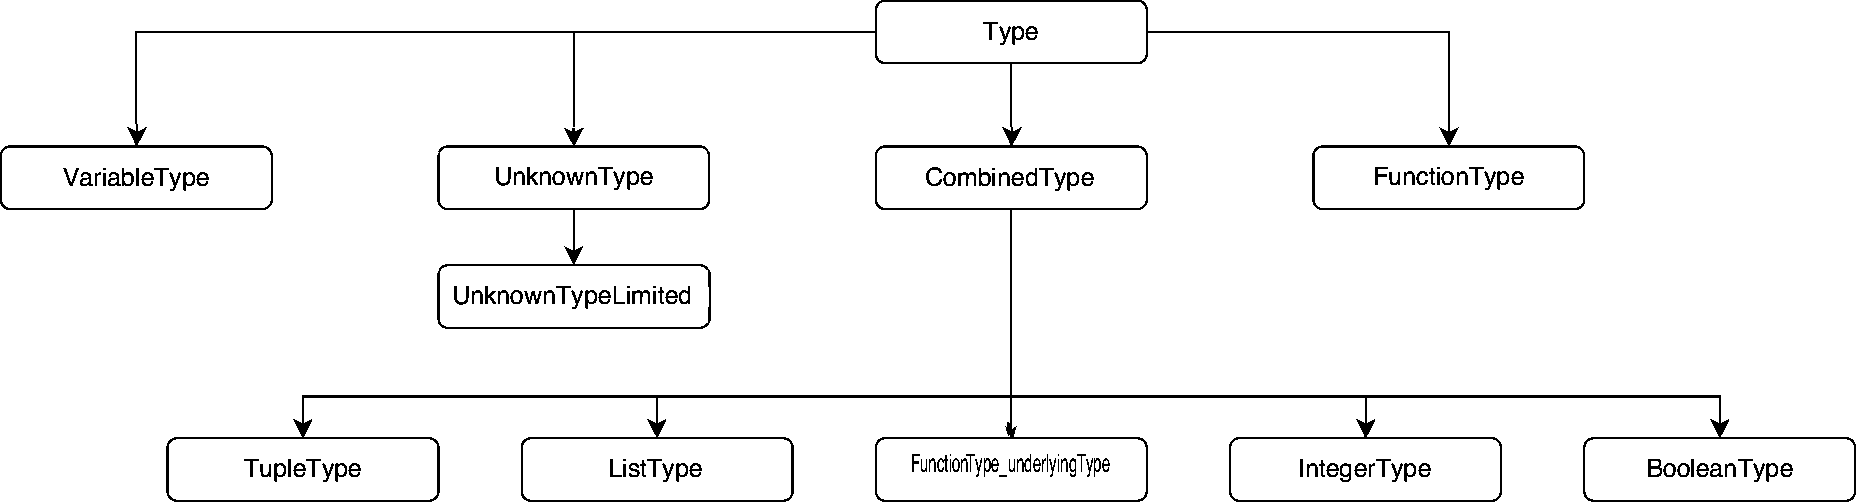
\includegraphics[width=\textwidth]{diagram.pdf}
			\vspace{0.2cm}

			\subsubsection{\texttt{Type} class}
				This class is abstract and corresponds to the normal scheme of a type. It has an unifying method, equality between types, an order, and some other handy functions.
			\subsubsection{Unknown type}
				This class represent a type we don't know anything about. At the first unifying with any type $t$, it will unify and merge the unknown type with $t$.
				It has an $UnknownTypeLimited$ variant, which is basically the same, but it's narrowing the type at some list of other types. In that case, we know more about the types.
			\subsubsection{CombinedType}
				This is the most important type. It's an abstract type that can contain any number of inner types: this is represented as a list of \cc{Type} (there are no constraints about the length of that list). When this type is extended, then it will create another type.

				A \cc{CombinedType} type $a$ unifies with another \cc{CombinedType} if and only if:
				\begin{itemize}
					\item $a$ and $b$ come from the same class;
					\item $a$ and $b$ have the same number of stored types;
					\item stored types in $a$ and $b$ have to unify pairwise. 
				\end{itemize}
			\subsubsection{TupleType}
				\cc{TupleType} extends \cc{CombinedType}. The constructor needs two arguments, a left type and a right type: it stores these types in its inner type list (from \cc{CombinedType}).
			\subsubsection{ListType}
				\cc{ListType} has a constructor taking just one type: the one contained in the list. It pushes this type in the inner type list (from \cc{CombinedType}).

			\subsubsection{FunctionType}
				The constructor takes any number of input argument types and one output type.

				It builds two  \cc{FunctionType_UnderlyingType} (extending \cc{CombinedType}): one with arguments and output types in the inner list, the other one only with inputs.

				Then, when unifying, it just uses underlying \cc{CombinedType} types own unifications with some twist to guess the output type in case of a generic function for example. 

			\subsubsection{Integer/Boolean type}
				Integer type does not contain any type information, the constructor takes nothing, and puts nothing on the inner list. Here if an integer type $a$ unifies with some type $b$, then $b$ is an integer, that's all.

				The exact same holds for booleans.

			\subsubsection{Type order}
				A type order is a tuple of two numbers. It measures the "concretness".
				
			\subsubsection{Type unification}
				Every type is immutable, in order to avoid conflicts with changing something somewhere and not elsewhere.

				When we unify a type $a$ with another one $b$, we obtain a list of replacements. A remplacement is a tuple of types: $(c,d)$ means $c$ has to be changed to $d$.

				Each time types are unified, we ask the linked context $ctx$ to unify everything itself. First, $ctx$ finds the context $ctx_{origin}$ where the variable to unify was declared first, then $ctx_{origin}$ browses all \cc{ParserRule} to apply the replacements.

			\subsubsection{Combined type unification}
				As described previously, $a$ can unify with $b$ only if it comes from the same class, has the same number of inside types, and inside types of $a$ and $b$ unify pairwise.

				Here, something bad can happen: if we unify $(Int, b)$ with $(a, a)$ (with $a$ an unkown type and $b$ a variable type), we want to deduce $(b, Int)$. But if we unify first $Int$ with $a$, we get $(a, Int)$. Then we unify $b$ with $a$ (which is now $Int$), and this is not working.

				To avoid that issue, I sort these unifications according type orders: we unify the less concrete ones in priority.

	\subsection{Add typing logic to the different \cc{ParserRule}s}
		I didn't want the type infering interfers with previous definitions of \cc{ParserRule}. Instead of overloading every \cc{ParseRule}, I just define a mapping from \cc{ParserRule} classes to typing logic.

		So basically, there is a big list of functions taking care of the typing logic of each \cc{ParserRule} that needs one.

		Some \cc{ParserRule} classes don't need any typing logic, for instance \cc{if} or \cc{while}. In this case, the type checker just digs into the \cc{ParserRule} definition and types check sub constructions. Hence, everything is verified, even if nothing is explicitely stated: this way, no any part of the program can be unchecked.


		I will explain some typing logic I find interesting.
		\subsubsection{Function declaration}
			Typing logic of function declaration is interesting because it needs to figure out if the function is well-typed, if it returns something, if the signature (if present) is making sense, etc.

			\paragraph{Pre treatment}
			First, I declare the identifier of the function in the context: this is useful because I want my compiler to support high order functions.

			Then I extract the arguments and the annotations to check if it is consistant (same numbers of parameters than annotations)

			\paragraph{Verifying returns paths}
				We need to ensure that the function actually returns for all different logical paths. For that, I use the following structure: \texttt{\{mabye: Ret[], concl: Ret[]\}}. Basically, \texttt{concl} represent some return statements like \texttt{if C then return A else return B}: it will be either A either B.  \texttt{concl} represents returns like \texttt{if C then return A}.

				I defined some compose functions taking two structures like that and outputing a new structure:
				\begin{lstlisting}
					type X = {maybe: Ret[], concl: Ret[]};
					let compose = (A:X, B: X) =>
						A.concl.length && B.concl.length ? {maybe: [...A.maybe, ...B.maybe], concl: [...A.concl, ...B.concl]} :
						A.concl.length == B.concl.length ? undefined : {maybe: [...A.maybe, ...B.maybe, ...A.concl, ...B.concl], concl: []};
				\end{lstlisting}

			\paragraph{Looking for type cycle dependencies}
				I build a dependency graph to check the dependencies between objects (functions or variables). If an ambiguous situation is spotted, then an error is raised and the user has to annote the function.

				Previously, if a cycle was found, I was using other return statements to guess the type, but that was quite buggy. Also, now I'm making a cycle dependency of every resource used inside a function, then I have no troubles when I type check the function body.

			\paragraph{Arranging the order of type check}
				The user is allowed to declare a function calling another function defined later on. That is not a problem, but if you ask the type checker to type the first function before typing the second one, it will fail.

				The previous step just eliminates situations where we have recursive type dependencies: hence it is not a graph but a tree, we don't have any cycle there. Then we can just order all the resources to type check the most needed things first.

				To do so, I use the tree of dependency and I just type check everything from the bottom of the tree to the top. Hence, I'm sure all dependencies will be satisfied. 

			\paragraph{Check if the output is making sense} Executing type checking modified the context, and hence, the output type. If the output type was given by annotation, I just need to check that the result is coherent. If there were no any annotations, then, I check if the output changed to a more concrete one.
		\subsection{Note}
			\cc{FunctionType} is just a normal type and can be used everywhere. \cc{VariableType} make polymorphism and generic programming possible.

			Hence, the type inference is strong enough to handle higher order functions.
	\section{SSM Code generation}
		Using everything done before in the type checker makes it quite easy.
		\subsection{Scopes}
			A scope correspond to all the (functions and variables) declarations of a function. Each declaration records exactly one new value on the stack and will be considered as the $n-th$ local value. 

			A value can either be a basic type (integer, boolean) either a composed type (tuple, list). A basic type is stored directly on the stack as a value, while a composed one store a pointer to the heap.

			Hence, when you access to a local variable, you can get either a pointer either a value, according the expected type (known at compiler time).

			But since we handle closure, we also need (that is explained later on) a way to store a simple value or a pointer to a complex value in the heap. Hence, a local variable can also be a pointer to a value.    

			The local variable positions are calculated by the \cc{Context}. A method in \cc{Context} gives information about any stored values, and compute the local position (relative to \texttt{MP}). It handle the case of parameters, local values, and exteral values linked by closures.

			The scope is organized on the stack in the following way (on the left are represented the local positions):

			\begin{center}
				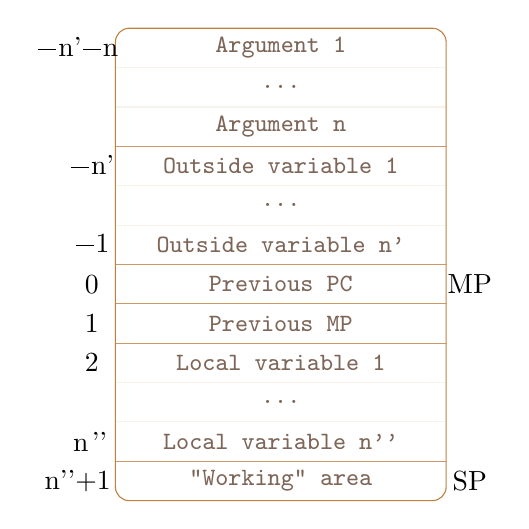
\begin{tikzpicture}[x=0.6cm,y=-0.5cm]
					\draw[rounded corners=5pt,thin, brown] (0,0) rectangle ++(7,12);
					\draw[rounded corners=5pt,thin, brown, opacity=0.1] (0,1) -- ++(7,0);
					\draw[rounded corners=5pt,thin, brown, opacity=0.1] (0,2) -- ++(7,0);
					
					\draw[rounded corners=5pt,thin, brown, opacity=0.8] (0,3) -- ++(7,0);

					\draw[rounded corners=5pt,thin, brown, opacity=0.1] (0,4) -- ++(7,0);
					\draw[rounded corners=5pt,thin, brown, opacity=0.1] (0,5) -- ++(7,0);

					\draw[rounded corners=5pt,thin, brown, opacity=0.8] (0,6) -- ++(7,0);
					\draw[rounded corners=5pt,thin, brown, opacity=0.8] (0,7) -- ++(7,0);
					\draw[rounded corners=5pt,thin, brown, opacity=0.8] (0,8) -- ++(7,0);

					\draw[rounded corners=5pt,thin, brown, opacity=0.1] (0,9) -- ++(7,0);
					\draw[rounded corners=5pt,thin, brown, opacity=0.1] (0,10) -- ++(7,0);
					\draw[rounded corners=5pt,thin, brown, opacity=0.8] (0,11) -- ++(7,0);

					\node at (3.5,0.5) {\ccd{Argument 1}};
					\node at (3.5,1.5) {\ccd{...}};
					\node at (3.5,2.5) {\ccd{Argument n}};

					\node at (3.5,3.5) {\ccd{Outside variable 1}};
					\node at (3.5,4.5) {\ccd{...}};
					\node at (3.5,5.5) {\ccd{Outside variable n'}};
					\node at (3.5,6.5) {\ccd{Previous PC}};
					\node at (3.5,7.5) {\ccd{Previous MP}};
					\node at (3.5,8.5) {\ccd{Local variable 1}};
					\node at (3.5,9.5) {\ccd{...}};
					\node at (3.5,10.5) {\ccd{Local variable n''}};
					\node at (3.5,11.5) {\ccd{"Working" area}};
					% \node at (3.5,2.5) {hey};
					\node at (7.5,6.5) {\cc{MP}};
					\node at (7.5,11.5) {\cc{SP}};

					\node at (-0.5,3.5) {\cc{-n'}};
					\node at (-0.8,0.5) {\cc{-n'-n}};
					\node at (-0.5,5.5) {\cc{-1}};
					\node at (-0.5,6.5) {\cc{0}};
					\node at (-0.5,7.5) {\cc{1}};
					\node at (-0.5,8.5) {\cc{2}};
					\node at (-0.5,10.5) {\cc{n''}};
					\node at (-0.8,11.5) {\cc{n''+1}};
				\end{tikzpicture}
			\end{center}
		\subsection{Closure support}
			When a function references a variable from some parent scope, I lift that variable to the heap: instead of having value (i.e. if it's an integer) or a pointer (i.e. if it's a list) in the local values, we will have a pointer to either a value or another pointer in the heap.
			That allows the value to be existing outside the local scope of some functions.

			Then, I use a structure to store these pointers along with the address of the closure.
		\subsection{Function pointer structure}
			This is basically just a package with some hidden parameters (the closure "outside variables") and with the PC.
			It has the following form:

			\begin{center}\label{funPointerStruct}
				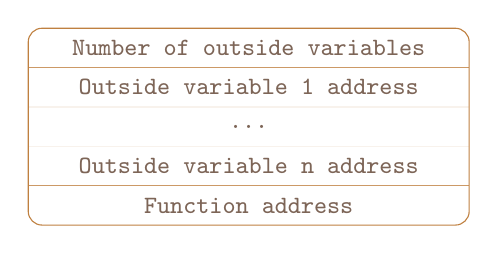
\begin{tikzpicture}[x=0.8cm,y=-0.5cm]
					\draw[rounded corners=5pt,thin, brown] (0,0) rectangle ++(7,5);
					\draw[rounded corners=5pt,thin, brown, opacity=0.8] (0,1) -- ++(7,0);
					\draw[rounded corners=5pt,thin, brown, opacity=0.1] (0,2) -- ++(7,0);
					\draw[rounded corners=5pt,thin, brown, opacity=0.1] (0,3) -- ++(7,0);
					\draw[rounded corners=5pt,thin, brown, opacity=0.8] (0,4) -- ++(7,0);
 
 					\node at (3.5,0.5) {\ccd{Number of outside variables}};
					\node at (3.5,1.5) {\ccd{Outside variable 1 address}};
					\node at (3.5,2.5) {\ccd{...}};
					\node at (3.5,3.5) {\ccd{Outside variable n address}};
					\node at (3.5,4.5) {\ccd{Function address}};
				\end{tikzpicture}
			\end{center}
		\subsection{Declaring a variable}
			There are two scenarios here:
			\paragraph{The variable is lifted to the heap} Here, we push on the stack the variable expression result - which is a single value (that can be a pointer or a value) - then we store it somewhere in the heap, and the resulting pointer will be our value, stored in locals (on the stack, then).
			\paragraph{The variable is not lifted} We do almost the same thing, but we skip the part where we put the resulting value on the heap. Here, we want the value to be stored directly on the stack.
		\subsection{Setting a variable}
			Again, two scenarios:
			\subsubsection{Lifted variable}
			Before setting a new value in some variable, we have to jump to the pointer specified by the variable in locals. Then, we can set the value. Here is the precise way of doing it:
			\begin{itemize}
				\item Push the new value on the stack;
				\item Save MP to RR;
				\item Load the variable pointer from locals;
				\item Set MP with top value of stack;
				\item Store in local (which is now the location pointed by the variable) the new value (which is on the stack);
				\item Restore registers.
			\end{itemize}
			\subsubsection{Not lifted variable}
				We just store the new value to locals.
		\subsection{Consulting a variable}
			To get a variable in position $p$, we need:
			\paragraph{If it's a lifted variable} Load using a local referencing an address (with \texttt{ldla $p$})
			\paragraph{Otherwise} Simply load a local value (with \texttt{ldl $p$})
		\subsection{Declaring a function}
			When we declare a function, we need to write on the stack the corresponding \texttt{Function pointer structure} (defined in \ref{funPointerStruct}), and to store it somewhere. After doing so, the resulting address will be on the locals, just like any other variable.
		\subsection{Calling a function}
			Let $f$ (a function pointer structure) be in the locals, then executing $f$ means:
			\begin{itemize}
				\item Load the value pointed by $f$: we retrive the number of outside variables $n$
				\item Load the $n+1$ next values after $f$: we retrive the outside variable pointers along with the program address
				\item Save the program address in RR (we don't want it to stay there on the stack)
				\item Push to the stack all the parameters
				\item Save current PC on the stack 
				\item Store the value of RR into PC (i.e. branching)  
			\end{itemize}
		\subsection{Global scope}
			I consider the global scope as a normal scope, as a normal function. So, basically, every top levels objects (function or variable declarations) behave as it was inside one big function.

			Hence, I don't need to rebuild some different dependencies analysis or anything: all objects belongs to some locals scope, but this "big fonction".

			Then, on the top level, on the global level, we have only one object, hence, no dependencies issue can occurs.
	\section{Conclusion}
		This course was very interesting for me, since it was the first time I built an actual compiler. I previously made some small parser to handle simple languages, but nothing serious.

		Working on that compiler was very interesting, even if it was quite time consuming. I feel much more confortable with how a compiler is working, now.
\end{document}